%%%%%%%%%%%%%%%%%%%%%%%%%%%%%%%%%%%%%%%%%%%
\subsection{Пример сложного вычислительного метода}
%%%%%%%%%%%%%%%%%%%%%%%%%%%%%%%%%%%%%%%%%%%
\begin{frame}
  \begin{figure}
    \centering
    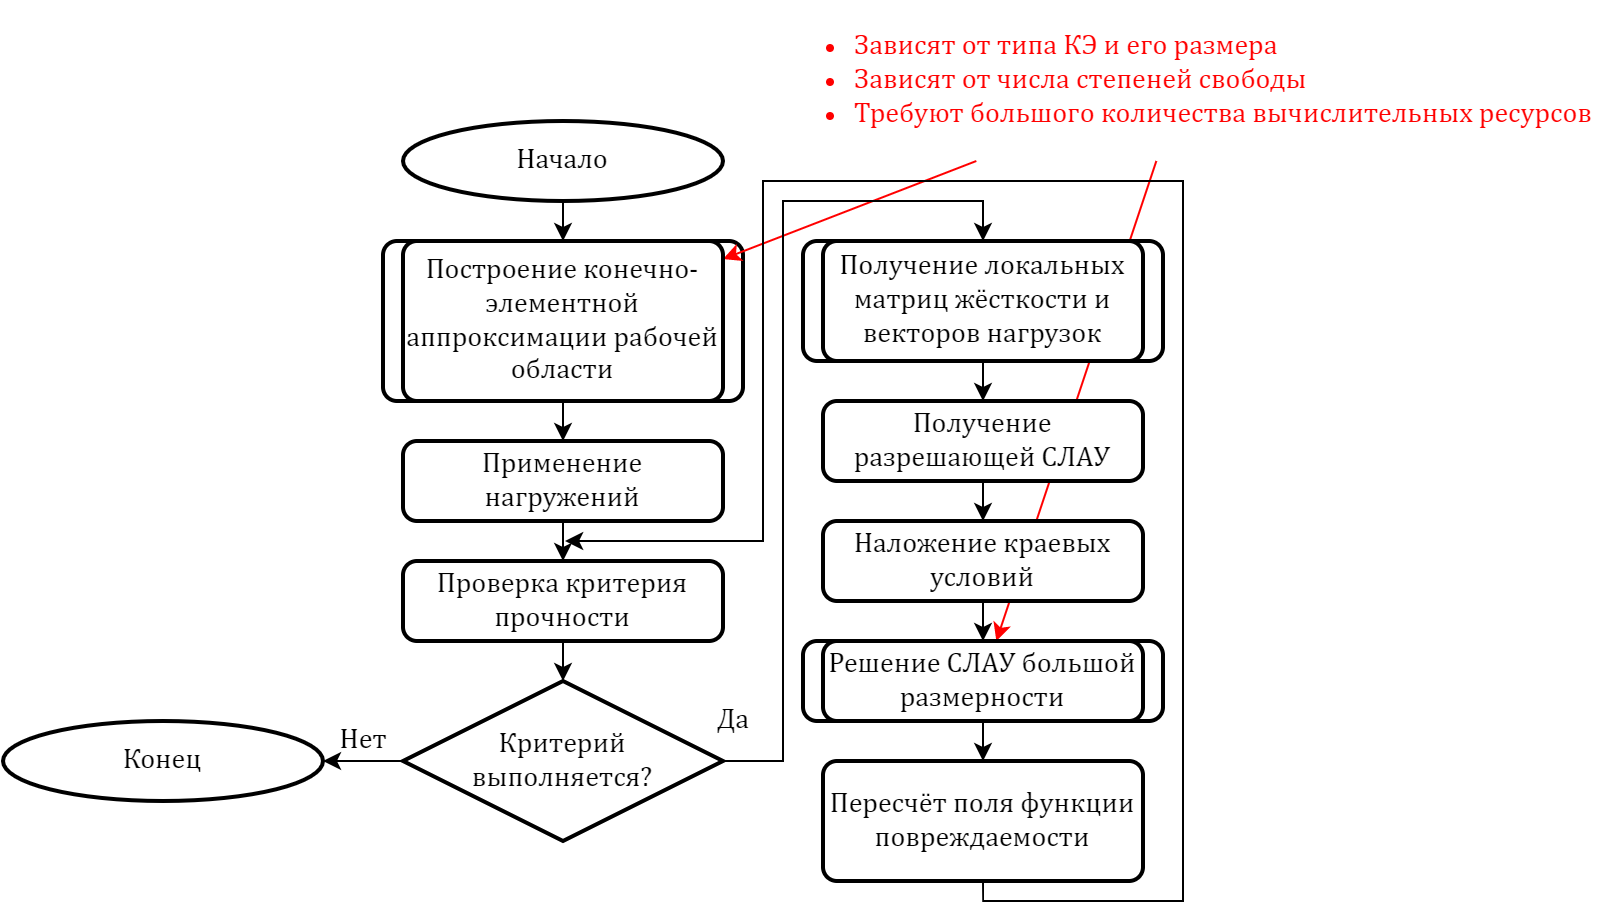
\includegraphics[width=\textwidth]{images/flowchart.fem.png}
    \caption{Применение метода конечных элементов для анализа прочности конструкции}
  \end{figure}

\end{frame}
% --------------------------------------------------------------------------- %
\subsection{Разработка трудоёмкого научно-технического ПО}
% --------------------------------------------------------------------------- %

\begin{frame}
  \begin{figure}
    \centering
    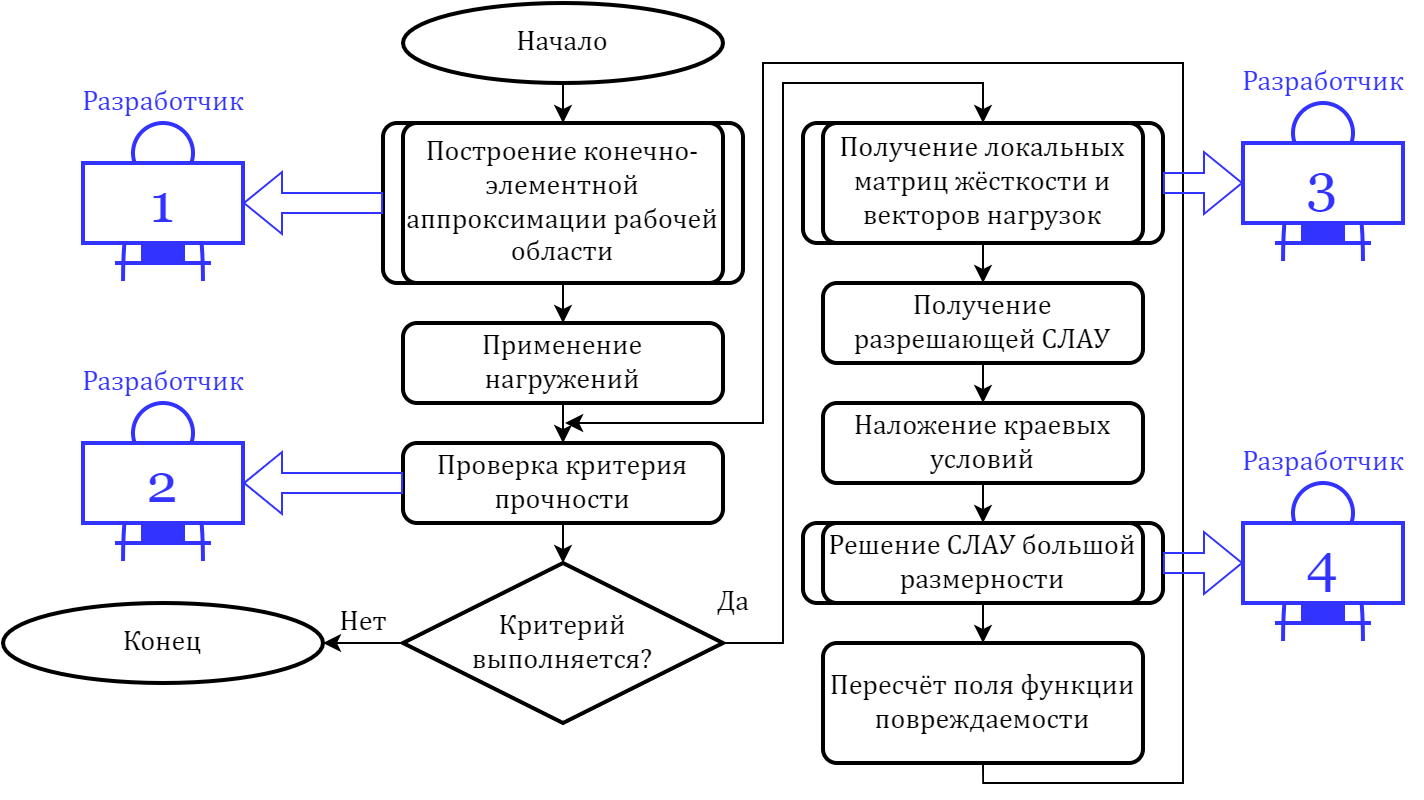
\includegraphics[width=\textwidth]{images/illustration.teamwork.png}
    \caption{Пример делегирования разработки отдельных этапов вычислительного метода}
  \end{figure}

  {\smaller[1]
  Делегирование реализации отдельных этапов реализуемого метода отдельным разработчикам положительно влияет на общее качество реализуемого ПО.
  }
\end{frame}

% --------------------------------------------------------------------------- %
\subsection{Современные средства, направленные на упрощение разработки}
% --------------------------------------------------------------------------- %
\begin{frame}



\end{frame}

% --------------------------------------------------------------------------- %
\subsection{Цели и задачи разработки}
% --------------------------------------------------------------------------- %
\begin{frame}

  \begin{block}{Цель}
    Разработать программные средства для создания и интерпретации графовых описаний вычислительных методов в программном каркасе comsdk.
  \end{block}

  \begin{block}{Задачи}
    \begin{enumerate}
      \item Провести сравнение объекта разработки с некоторым аналогичным.
      \item Сформировать требования к алгоритму, выполняющему этапы алгоритма по его описанию, составленному по методологии GBSE.
      \item Спроектировать структуры данных для описания и представления описаний алгоритмов и их элементов в программном каркасе comsdk.
      \item Разработать алгоритм обхода графовых моделей с использованием спроектированных структур данных.
      \item Представить интерфейсы или реализации разработанных алгоритмов и структур данных на языке С++.
    \end{enumerate}
  \end{block}

\end{frame}


